\documentclass{article}
\usepackage{graphicx}
% for use of german language in a document
\usepackage[utf8]{inputenc} % this is needed for umlauts
\usepackage[ngerman]{babel} % this is needed for umlauts
\usepackage[T1]{fontenc}    % this is needed for correct output of umlauts in pdf


\pagestyle{empty}

\begin{document}

\section*{Arbeitsgruppe: Einfache endliche Gruppen}

Im kommenden Semester soll eine Arbeitsgruppe zum Thema einfache endliche Gruppen angeboten werden. Ziel ist es, an interessante Gruppen anhand des Buches CFSG\footnote{Classification Theorem for Finite Simple Groups} heranzuführen und die damit verbunden algebraischen Strukturen zu studieren.

\paragraph{Inhalt:}
Zunächst wird es am Anfang des Semesters es eine kleine Auffrischung zu sehr grundlegenden Aussagen und Sätzen der Gruppentheorie geben.
Danach wird ein Großteil des Stoffes konkrete Beispiele von Gruppen sein. Im Wesentlichen soll das Seminar auf dem Buch `The Finite Simple Groups' von Robert Wilson
basieren (aus dem wir wahrscheinlich nur einen Bruchteil schaffen werden). Der Inhalt des Seminars soll durch die Hörerschaft mitbestimmt werden.

\begin{figure}[htb]
    \centering
    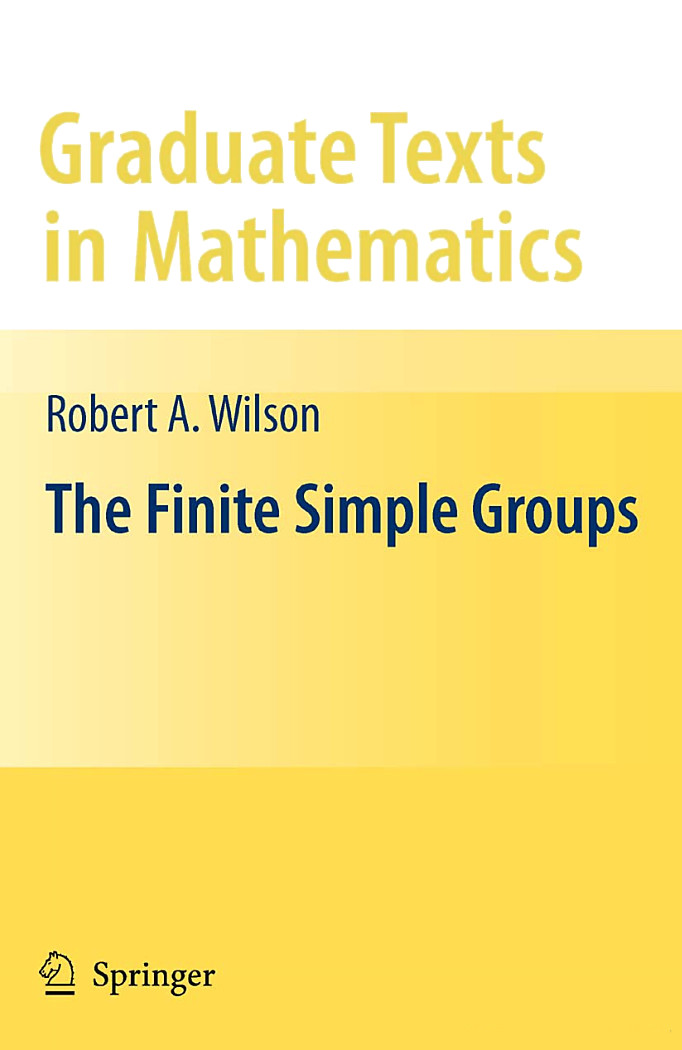
\includegraphics[width=0.4\textwidth]{FSG.jpg}
\end{figure}

\paragraph{Gestaltung:} Optimal wäre es, wenn die Teilnehmer die Arbeitsgruppe selbst durch eigene Vorträge beleben würden.
Auch Studentinnen und Studenten höherer Semester, die sich mit der Thematik schon ein wenig auseinandergesetzt haben, sind also willkommen.
Grundsätzlich soll die Vermittlung des Stoffes jedoch derart konzipiert sein, dass dieser für Bachelorstudenten ab dem dritten Semester verständlich ist.
Ich stehe bei Rückfragen gerne per Email zur Verfügung ({\tt jakob.schneider@tu-dresden.de}).


\begin{flushright}
    \today,\\
    Jakob Schneider  
\end{flushright}


\end{document}